\subsection{Sparsely distributed sensor arrays}
Sparsely distributed sensor arrays refer to layouts that limit the number of available sensors either by environmental parameters or by design. This limits the information that can be gathered about the detectable object, or reduces the number of different objects that can be distinguished. To compensate this limitation a number of interpolation methods can be used that take into account our knowledge about the position and shape of the electrodes used in the current setup. One example for this sparse distribution is the previously presented Thracker system that uses only four electrodes to acquire a hand position and detect gestures at certain positions \cite{Wimmer2007a}. In this section I will present two different contributions - a new method to recognize single-hand gestures in free-air using just six different sensors and an indoor localization system based on a coarse grid of wire electrodes that can be hidden below different floor surfaces.
\subsubsection{3D location tracking and gesture interaction}
 \begin{figure}[h]
\centering
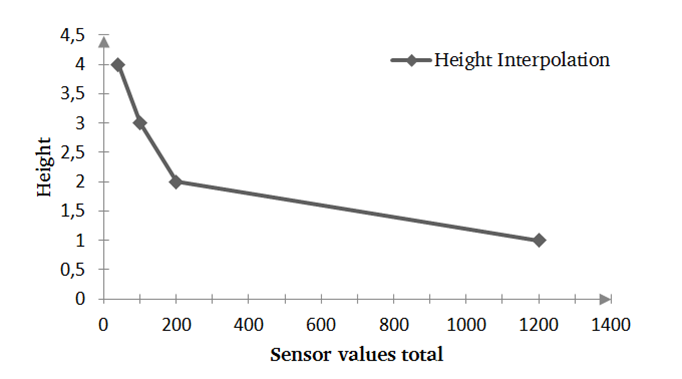
\includegraphics[width=0.6\textwidth]{images/magicbox_data_zaxis}
\caption{Piecewise linear hand distance estimation \cite{Braun2011MultiInputDevice}}
\label{fig:magicbox_data_zaxis}
\end{figure}
Gesture recognition can comprise a large number of different body movements, including sign language that uses movements and position of hands and fingers, the posture of the whole body, or as in our case the movement of the hand in three dimensions. This requires two distinct processing steps. At first it is necessary to precisely localize the position of the hand in the interaction space. Afterwards, a time series of theses positions has to be analyzed and attributed to different gestures. The localization method was first presented in a publication from 2011 \cite{Braun2011MultiInputDevice}. The static gesture recognition method used there was later extended by adapting algorithms used to detect mouse gestures for movements in three dimensions \cite{braun2013capacitive}. 
The first data processing step is the planar localization of the hand, following a weighted average algorithm, whereas $n$ is the number of sensors, $(x_i, y_i)$ the location of the electrode centers and $v_i$ the value of the given sensor.
\begin{align}
\overline{x}&=\frac{\sum^n_{i=1}{v_i\cdot x_i}}{\sum^n_{i=1}{v_i}} & \overline{y}&=\frac{\sum^n_{i=1}{v_i\cdot y_i}}{\sum^n_{i=1}{v_i}}
\end{align}
In order to calculate the distance of the hand from the plane we are using a piecewise linear interpolation, that resembles the response curve of a single sensor \cite{Braun2011MultiInputDevice}. In this case four different thresholds $t_i$ are used to calculate the proximity, based on the sum of sensor values. $t_1$ indicates the closest distinguishable proximity, e.g. touch, with all higher value sums associated to this. $t_4$ represents the maximum distance in which the sensors can detect a hand. One example with fixed points at values 40, 100, 200 and 1200 is shown in Figure \ref{fig:magicbox_data_zaxis}.
\begin{figure}[h]
\centering
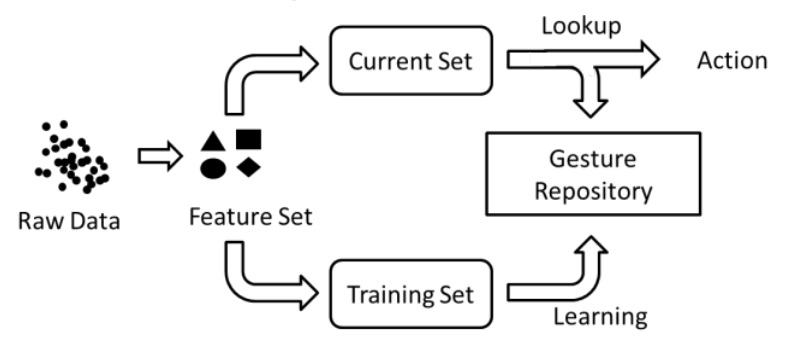
\includegraphics[width=0.7\textwidth]{images/gesture_by_example}
\caption{Principle components of a learning by example recognition framework \cite{braun2013capacitive}}
\label{fig:gesture_by_example}
\end{figure}
Initially a static gesture recognition method was implemented that used a series of five subsequent locations and simple heuristics to determine a small number of gestures. Thus, a generic gesture recognition module was created, based on learning by example \cite{braun2013capacitive}. The general functionality of a gesture recognition framework that is using learning by example is shown in Figure \ref{fig:gesture_by_example}. A feature set is extracted from incoming raw data. Collections of these are distinguished into training sets that are used to associate certain features to given gestures. After a learning process the current feature sets, acquired on-the-fly, are tested against the training sets in a repository. These look-ups can lead to successful gesture recognition and association to certain actions. This association method is also called classification. There are numerous approaches, e.g. neural networks (NN) or support vector machines (SVM).

\subsubsection{Large-area location tracking}
There are several systems that use capacitive proximity sensing to track the location of one or more persons in an environment. A common challenge in large areas is achieving a suitable coverage with electrodes at all positions. Lauterbach et al. overcome this problem in their SensFloor system by integrating sensors and electrodes in an underlay that can be placed below the upper layer of the floor \cite{lauterbach2009}. TileTrack, the system developed by Valtonen et al. requires large emitter electrodes under the floor and receivers placed in the walls \cite{Valtonen2009a}. To overcome this limitation they later integrated receivers into different pieces of furniture.

While SensFloor allows to cover large areas by having the sensing electrodes near all surface areas, a limitation is maintenance. If a sensor breaks below the floor covering it is difficult to replace. TileTrack in its initial installation requires proximity to walls, or later to specific pieces of furniture that are in the environment. This is difficult to guarantee in many instances and requires an initial calibration of the environment, according to placement of the furniture.

\begin{figure}[h]
\centering
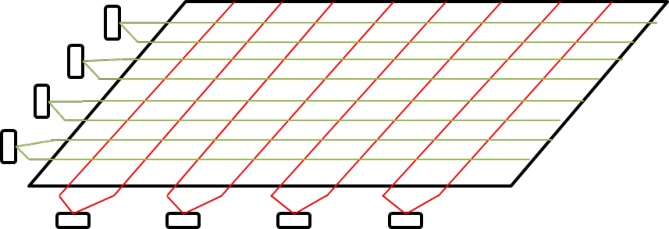
\includegraphics[width=0.8\textwidth]{images/capfloor_concept}
\caption{Wire electrode grid below floor cover attached to sensors on the border}
\label{fig:capfloor_concept}
\end{figure}

I proposed a system based on a rectangular grid of long wire electrodes that are placed below the top floor cover, with sensors attached at the edge of the area, e.g. in skirting boards \cite{Braun2012CapFloor}. As the system is based on loading mode there is no need for dedicated receivers, but instead relies solely on the electrodes below the floor. The system is akin to a larger variety of projected capacitive touch screens that are partially also using grid layouts \cite{BarrettScreen}. 
\begin{figure}[h]
\centering
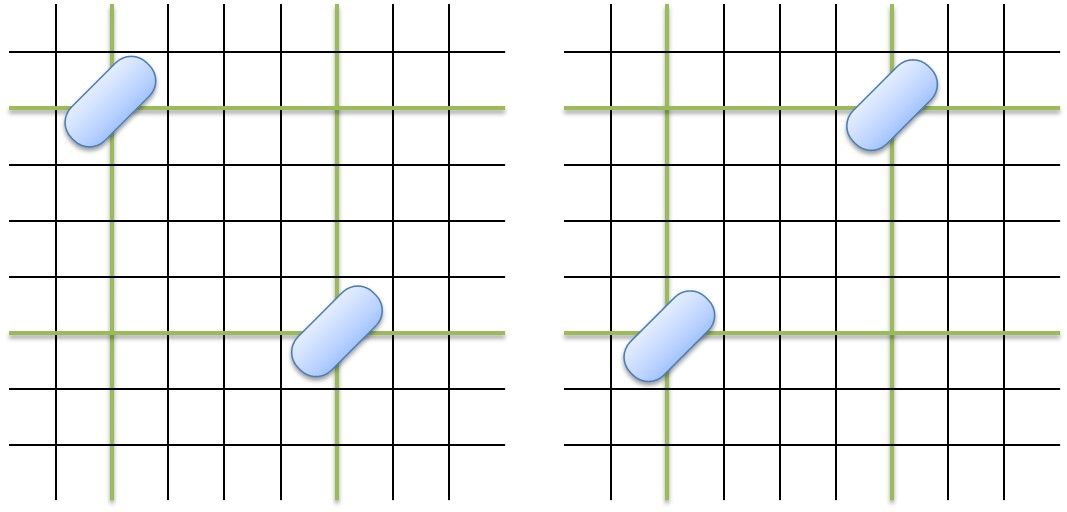
\includegraphics[width=0.8\textwidth]{images/capfloor_ghosting}
\caption{Two potential person locations resulting in same sensor readings (green indicates active electrodes}
\label{fig:capfloor_ghosting}
\end{figure}
Using long, straight wire electrodes have different effects on the measurement. One effect of this is the limited detection distance that is not comparable to large plate electrodes. Particularly if thick floor covers are used the grid has to be fairly dense. Another effect is the sensitivity towards noise and influence from outside electric fields. Therefore the system requires preprocessing to reduce the noise and achieve a more robust high-level data processing. In order to localize persons the system uses an adapted weighted average algorithm, similar to the variety presented in the previous section. Each electrode is considered to only have a single coordinate in either $x$ or $y$ direction, allowing to easily calculate the center-of-gravity. However, it can occur that only two electrodes are active at a certain point in time, while two persons are present and too far away from any other electrode to be detected. In these cases there is a certain ambiguity as each $(x,y)$ value combination can result in two potential intersection points, as shown in Figure \ref{fig:capfloor_ghosting}. To overcome this problem it is possible to either use a mix of sending and receiving electrodes operating in shunt mode and specific measurement cycles. Another option is to analyze the time-series of previous locations to discard unlikely positions.
\begin{figure}[h]
\centering
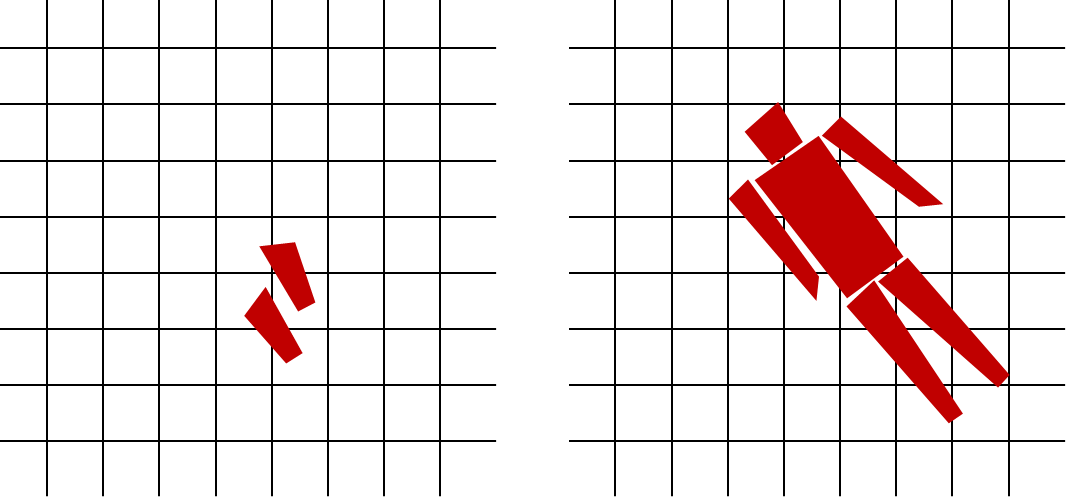
\includegraphics[width=0.8\textwidth]{images/floor_shapes}
\caption{Shapes of a standing and lying person on top of the CapFloor grid}
\label{fig:capfloor_shapes}
\end{figure}
Similar to SensFloor the concept also supports detecting additional information about the persons present, most notably fall detection. This is based on a time-series analysis of aggregated values of the sensors that are currently detecting an object. This method is using the assumption that the overall sensor response is roughly equivalent to the shape of the object that is closest to the surface, resulting in a higher capacitance of the overall system, similar to the plate capacitor model. This effect is shown in Figure \ref{fig:capfloor_shapes}. The sum $s$ of all n sensor values $r$ is the closest equivalent to the system capacitance and therefore a viable measure. If the overall value is beyond a certain threshold $v_l$ we can consider a lying person $p_l$.
\begin{align}
s&=\sum^n_{i=0}{r_i} & p_l&=\left\{ \begin{array}{c}
1,\ \ \ s\ge v_l \\ 
0,\ \ \ s<v_l \end{array}
\right.
\end{align}
In order to increase the robustness this threshold has to be exceeded for a certain amount of time $t_m$. In consequence a fall $f$ is detected if the following equation is 1.
\begin{equation}
f=\prod^{t_m}_{j=0}{p_{l,t_j}}
\end{equation}